\documentclass{beamer}
\mode<presentation>
{
  \usetheme{Warsaw}      % or try Darmstadt, Madrid, Warsaw, ...
  \usecolortheme{beaver} % or try albatross, beaver, crane, ...
  \usefonttheme{default}  % or try serif, structurebold, ...
  \setbeamertemplate{navigation symbols}{}
  \setbeamertemplate{caption}[numbered]
  \setbeamertemplate{footline}[frame number]
}


\usepackage[english]{babel}
\usepackage[utf8]{inputenc}
\usepackage{pgfpages}
\usepackage{algorithm}
\usepackage{color}
\usepackage[noend]{algorithmic}

\title {Real-Time Systems}
\subtitle {The Space of Feasible Execution Times for Asynchronous Periodic Task
Systems using Definitive Idle Times}
\author{Thomas~Chapeaux~\inst{1}~\inst{2} \and Paul~Rodriguez~\inst{1}~\inst{2} \and Laurent~George~\inst{2} \and Joël~Goossens~\inst{1}}
\institute[shortinst]{\inst{1} Université Libre de Bruxelles \\ Belgium \and %
                      \inst{2} ECE Paris \\ France}
\date{July 2013}

\newcommand{\dbf}[1]{\operatorname{dbf}(#1)}

\begin{document}

\maketitle{}

\begin{frame}
    \tableofcontents[hideallsubsections]
\end{frame}

\section{Introduction}

\begin{frame}
    \tableofcontents[currentsection, hideallsubsections]
\end{frame}

% 	\subsection{Real-time systems}

	\begin{frame}{Model}
  \begin{block}{Real-Time Systems}
  Systems with timeliness constraints. (e.g. ABS, VOD, etc)
  \end{block}
  \textbf{Model:} $\tau$ set of $n$ tasks $\tau_i = (O_i, C_i, D_i, T_i)$ generating jobs $J_{i,j}$
      \begin{itemize}
      \item $O_i$ : arrival of the first job
      \item $C_i$ : execution time
      \item $D_i$ : relative deadline
      \item $T_i$ : time between two job arrivals
    \end{itemize}
  We consider periodic systems with constrained deadline on uniprocessor platforms.

  \begin{columns}[c] % the "c" option specifies center vertical alignment
  \column{.4\textwidth}
\begin{center}
\begin{tabular}{|r|c|c|c|c|}
 \hline
  & $O_i$ & $C_i$ & $D_i$ & $T_i$ \\
 \hline
 $\tau_1$ & 1 & 2 & 6 & 10\\
 \hline
 $\tau_2$ & 0 & 3 & 5 & 5\\
 \hline
\end{tabular}
\end{center}

  \column{.6\textwidth} % column designated by a command
\begin{figure}[h]
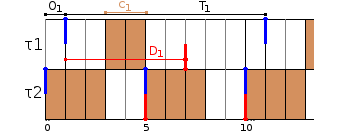
\includegraphics[width=0.7\textwidth]{figs/RTsystem_example.png}
\label{fig:llf}
\end{figure}
  \end{columns}


\end{frame}

    \subsection{Feasibility}

    \subsection{Motivation}

    \begin{frame}{Motivation}

        \begin{block}{Feasibility}
        A task set is said to be \textbf{feasible} if there exists a schedule such that every job in the task set completes before its deadline is reached.
        \end{block}


        \begin{itemize}
            % \begin{columns}[c]
            % \column{.1\textwidth}
            % \column{.4\textwidth}
            %     \begin{tabular}{|r|c|c|c|c|}
            %      \hline
            %       & $O_i$ & $C_i$ & $D_i$ & $T_i$ \\
            %      \hline
            %      $\tau_1$ & 1 & 2 & 6 & 10\\
            %      \hline
            %      $\tau_2$ & 0 & 3 & 5 & 5\\
            %      \hline
            %     \end{tabular}
            % \column{.5\textwidth}
            %     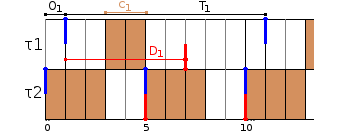
\includegraphics[width=\textwidth]{figs/RTsystem_example.png}
            % \end{columns}
            \item When implementing a system on different platform, the $C_i$ values may vary. How can we efficiently check if a system is feasible on a given platform?

            \item Most feasibility tests assume specific values of the $C_i$, which means that they must be applied once for each candidate platform.

            \item Our solution is to provide a description of the space of feasible execution times which can be  used to efficiently test any platform.
        \end{itemize}
    \end{frame}

    \subsection{C-space}

    \begin{frame}{Definition of the C-space}
        \begin{block}{C-space}
            The \textbf{C-space} of a task system $\tau$ is a region of $n$ dimensions (where each dimension denotes the possible $C_i$ of a task of $\tau$) such that for any point $C = \{ C_1, \cdots, C_{n}\}$ in it, $\tau$ is feasible.
        \end{block}

\begin{columns}[c]
    \column{0.5\textwidth}
        \begin{itemize}
            \item A region of $\mathbb{N}_0^n$ such as the C-space is described by a set of parametric linear constraints on the $C_i$.
            \item Example:
            \begin{tabular}{|r|c|c|c|c|}
             \hline
              & $O_i$ & $C_i$ & $D_i$ & $T_i$ \\
             \hline
             $\tau_1$ & 1 & ? & 6 & 10\\
             \hline
             $\tau_2$ & 0 & ? & 5 & 5\\
             \hline
            \end{tabular}
        \end{itemize}
    \column{0.5\textwidth}
        \begin{center}
        \begin{figure}
            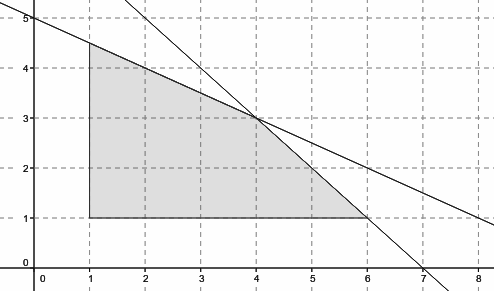
\includegraphics[width=0.9\textwidth]{figs/cspace_example_2.png}
            \caption{C-space containing 17 possible $C_i$ values}
        \end{figure}
        \end{center}

    \end{columns}
    \end{frame}

    \begin{frame}{C-space of synchronous systems}

    \begin{itemize}
        \item The authors of \cite{george2009characterization} obtain an efficient description of the C-space of synchronous systems based on the DBF test\cite{baruah1990algorithms}, a necessary and sufficient condition of feasibility for constrained deadline systems.
        \item However, synchronous systems are a worst-case with regards to feasibility, i.e. some unfeasible synchronous systems become feasible if specific offsets are added. In the literature (e.g. \cite{goossens2003scheduling}), the benefits of offsets are confirmed.
        \item This motivates a description of the C-space for asynchronous systems.

    \end{itemize}


% a necessary and sufficient condition of feasibility:$$\dbf{t_1, t_2} = \sum_{i=1}^{n} n_i(t_1, t_2) \, C_i \leqslant t_2 - t_1 \; \; \forall t_1 \leq t_2$$
%         where $n_i(t_1, t_2)$ is the number of jobs of $\tau_i$ in the interval $[t_1, t_2]$.

%     ~\\

%     The description is given by the DBF test on intervals $[0, t]$, where $t$ is a deadline and $0 < t \leqslant H$ (with $H = LCM(T_i)$).

%     ~\\

%     The remaining redundancies are removed by an algorithm based on the simplex (with exponential worst-case complexity).

    \end{frame}

	\subsection{Our work}

	\begin{frame}{Our work}

	In the article, we
    \begin{itemize}
        \item Introduce the notion of \textbf{First Periodic Definitive Idle Times}, which provides a study interval independent of the execution times.
        \item Extend the description of the C-space for asynchronous periodic constrained deadline systems
        \item Quantify the feasibility gain of random offsets in terms of C-space volume ratio.
    \end{itemize}

	\end{frame}

\section{First Periodic DIT}

    \begin{frame}
        \tableofcontents[currentsection, hideallsubsections]
    \end{frame}

	\subsection{Definition}

	\begin{frame}{Definition of the FPDIT}
        \begin{block}{Definitive Idle Time}
            A \textbf{definitive idle time} (DIT) \cite{lipariaverage} is a time $t$ such that every job released strictly before instant $t$ has its absolute deadline before or at instant $t$.
        \end{block}

        \begin{block}{First Periodic DIT}
			The \textbf{first periodic DIT} (FPDIT) of a system is the earliest DIT occurring
			strictly after $O_{max}$.
		\end{block}

        \begin{columns}[c]
        \column{0.5\textwidth}

        \includegraphics<1>[width=\textwidth]{figs/DIT_example.png}
        \includegraphics<2>[width=\textwidth]{figs/DIT_example_2.png}

        \column{0.5\textwidth}

        The FPDIT is the smallest $t_d$ such as:
       \[
            \begin{array}{l}
                \forall \tau_i \in \tau, \exists a_i \in [D_i,T_i] \; :\\
                \left\{
                    \begin{array}{l}
                        t_d > O_i \\
                        t_d - O_i \equiv a_i \; (mod \; T_i)
                        \\
                    \end{array}
                \right.
            \end{array}
        \]
        \end{columns}

	\end{frame}

    \subsection{Possible non-existence}

    \begin{frame}{Possible non-existence}

    \begin{itemize}
        \item In asynchronous systems, it is possible for a system to not have any FPDIT. Example:
        \begin{center}
            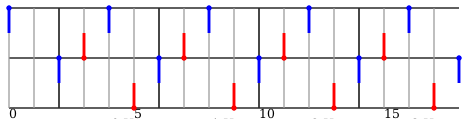
\includegraphics[width=.6\textwidth]{figs/nofpdit_example.png}
        \end{center}
        \item In fact, a system has a FPDIT if and only if the following condition is fulfilled for some value of $a_i$:

            \[
                a_i + O_i \equiv a_j + O_j \; (\operatorname{mod} \; \operatorname{gcd}(T_i,
                T_j)) \; \forall i,j
            \]

        \item Note that in synchronous systems ($O_i = 0 \; \forall i$), the hyperiod $H = LCM(T_i)$ is always a DIT.
    \end{itemize}

    \end{frame}

    \subsection{Frequency of existence}

    \begin{frame}{Frequency of existence of the FPDIT}

    \begin{columns}[c]
        \column{0.6\textwidth}

        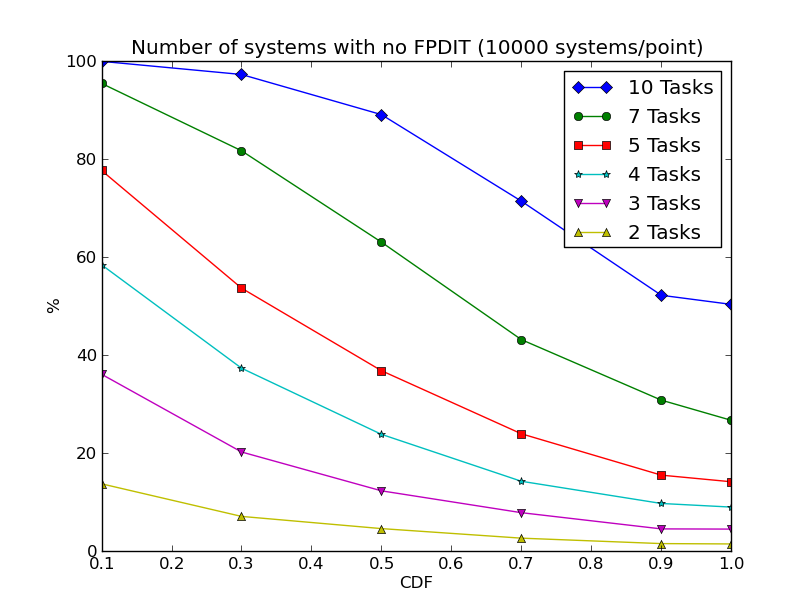
\includegraphics[width=1\textwidth]{figs/nofpdit_5.png}

        \column{0.4\textwidth}
        Systems were generated by
        \begin{itemize}
            \item Choosing $T_i$ in [5, 20]
            \item Choosing $O_i$ in [0, $H$]
            \item Choosing $D_i$ in [$T_i - CDF * T_i$, $T_i$]
        \end{itemize}

    \end{columns}

    FPDIT are less frequent in systems with a high number of tasks or a low CDF.

    \end{frame}

\section{C-space of asynchronous systems}

    \begin{frame}
        \tableofcontents[currentsection, hideallsubsections]
    \end{frame}

    \subsection{Initial description}

	\begin{frame}{Initial description}
		The C-space is accurately described by the following infinite number of constraints:

        $$\dbf{t_1, t_2} = \sum_{i=1}^{n} n_i(t_1, t_2) \, C_i \leq t_2 - t_1 \; \forall t_1 \leqslant  t_2$$
        where $n_i(t_1, t_2)$ is the number of jobs of $\tau_i$ whose release time and deadline are both strictly included the interval $[t_1, t_2]$.

        ~\\

        Based on previous results, a sufficient description is given by intervals $[t_1, t_2]$ where
        \begin{itemize}
            \item $t_1$ is an arrival
            \item $t_2$ is a deadline
            \item $0 \leqslant t_1 < t_2 \leqslant O_{max} + 2 \cdot H$ (where $H = LCM(T_i)$)
        \end{itemize}
	\end{frame}

    \subsection{Removing redundancies}

    \begin{frame}{Using the FPDIT}

        If the FPDIT exists, we can use the constraints given by the DBF test on intervals $[t_1, t_2]$ such that
        $$t_d \leqslant t_1 < t_2 \leqslant t_d + H$$
        which is a smaller interval than $[0, O_{max} + 2 \cdot H]$

    \end{frame}

    \begin{frame}{Redundancy as an ILP}

    We can define the redundancy of a linear constraint with regards to the set of $k$ linear constraints as an Integer Linear Problem.

        \begin{itemize}
            % \item If $z \leqslant t_2 - t_1$, the constraint is redundant
            % \item Can be solved with a branch-and-bound approach
            \item Each constraint of the set must be tested
            \item The worst-case complexity of each test is exponential in $k$
            \item In the paper, we propose a two-pass approach to reduce the number of constraints.
        \end{itemize}

    \end{frame}
    \subsection{Example}

    \begin{frame}{Example (I)}
        \[
        \begin{array}{|r|c|c|c|c|}
         \hline
          & O_i & C_i & D_i & T_i \\
         \hline
         \tau_2 & 0 & C_2 & 2 & 5\\
         \hline
         \tau_1 & 8 & C_1 & 7 & 15\\
         \hline
        \end{array}
        \]

        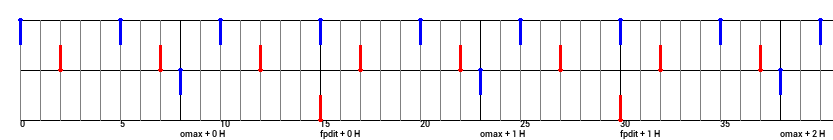
\includegraphics[width=\textwidth]{figs/CspaceExampleArrDead.png}

        \begin{itemize}
            \item $H = 15$
            \item The FPDIT happens at $t_d = 15$
            \item Our study interval is $[15, 30]$ which yields 11 constraints
            \item Without the FPDIT, the interval would be $[8, 38]$ (57 constraints)
        \end{itemize}
    \end{frame}

    \begin{frame}{Example (II) ILP first pass}

    \begin{columns}[c]
    \column{.45\textwidth}
        \begin{center}
            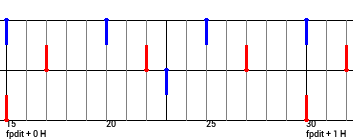
\includegraphics[width=\textwidth]{figs/CspaceExampleArrDead_restricted.png}
        \end{center}

        The DBF test:
        $$\sum_{i=1}^{n} n_i(t_1, t_2) \cdot C_i \leqslant t_2 - t_1 \; \; \forall t_1 \leq t_2$$

    \column{.55\textwidth}
        \[
        \left\{
            \begin{array}{cccccccc}
                0 & C_1 & + & 1 & C_2 & \leqslant & 17 - 15 & (x) \\
                \pause
                    \color{gray} 0 &
                    \color{gray} C_1 &
                    \color{gray} + &
                    \color{gray} 2 &
                    \color{gray} C_2 &
                    \color{gray} \leqslant &
                    \color{gray} 22 - 15 & \\
                \pause
                    \color{gray} 0 &
                    \color{gray} C_1 &
                    \color{gray} + &
                    \color{gray} 3 &
                    \color{gray} C_2 &
                    \color{gray} \leqslant &
                    \color{gray} 27 - 15 & \\
                \pause
                1 & C_1 & + & 3 & C_2 & \leqslant & 30 - 15 & (x) \\
                \pause
                    \color{gray} 0 &
                    \color{gray} C_1 &
                    \color{gray} + &
                    \color{gray} 1 &
                    \color{gray} C_2 &
                    \color{gray} \leqslant &
                    \color{gray} 22 - 20 & \\
                    \color{gray} 0 &
                    \color{gray} C_1 &
                    \color{gray} + &
                    \color{gray} 2 &
                    \color{gray} C_2 &
                    \color{gray} \leqslant &
                    \color{gray} 27 - 20 & \\
                1 & C_1 & + & 2 & C_2 & \leqslant & 30 - 20 & (x) \\
                    \color{gray} 0 &
                    \color{gray} C_1 &
                    \color{gray} + &
                    \color{gray} 1 &
                    \color{gray} C_2 &
                    \color{gray} \leqslant &
                    \color{gray} 27 - 23 & \\
                1 & C_1 & + & 1 & C_2 & \leqslant & 30 - 23 & (x) \\
                    \color{gray} 0 &
                    \color{gray} C_1 &
                    \color{gray} + &
                    \color{gray} 1 &
                    \color{gray} C_2 &
                    \color{gray} \leqslant &
                    \color{gray} 27 - 25 & \\
                    \color{gray} 0 &
                    \color{gray} C_1 &
                    \color{gray} + &
                    \color{gray} 1 &
                    \color{gray} C_2 &
                    \color{gray} \leqslant &
                    \color{gray} 30 - 25 & \\
            \end{array}
        \right.
        \]
    \end{columns}
    \end{frame}

    \begin{frame}{Example (II)}

    We remove the remaining redundancies with a second exhaustive pass:
    $$
        \left\{
            \begin{array}{cccccc}
                & & & C_2 & \leqslant & 2 \\
                C_1 & + & & C_2 & \leqslant & 7
            \end{array}
        \right.
    $$

    The C-space of the corresponding synchronous system is:
    $$
    \left\{
      \begin{array}{cccccc}
        & & & C_2 & \leqslant & 2 \\
        C_1 & + & 2 & C_2 & \leqslant & 7
      \end{array}
    \right.
    $$

    \begin{columns}[c]

    \column{0.5\textwidth}

    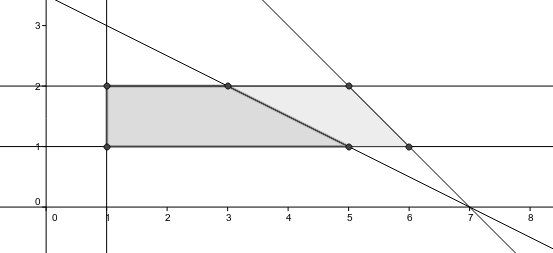
\includegraphics[width=\textwidth]{figs/cspace_example.png}

    \column{0.5\textwidth}

    The offsets allow three more $C_i$ values to be feasible.

    \end{columns}

    \end{frame}

\section{Feasibility gain of random offsets}

    \begin{frame}
        \tableofcontents[currentsection, hideallsubsections]
    \end{frame}

    \begin{frame}{Experiment}

        Because the synchronous release is known to be the worst-case feasibility-wise, we know that random offset can only improve the feasibility of a system.

        ~\\

        We express this feasibility gain given as the ratio

        $$\frac{V(\tau)}{V(\tau')}$$

        Where
        \begin{itemize}
            \item $\tau$ is a synchronous system
            \item $\tau'$ is $\tau$ with added offsets
            \item $V(\tau)$ is the size of the C-space of $\tau$
        \end{itemize}

    \end{frame}

    \begin{frame}{Result}

        \begin{columns}[c]

        \column{0.5\textwidth}

            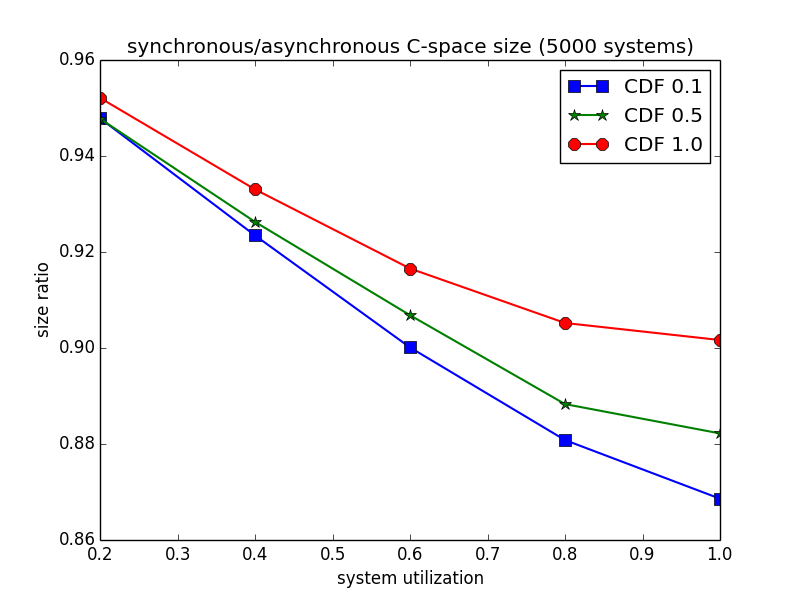
\includegraphics[width=1.2\textwidth]{figs/sizeratio.png}

        \column{0.5\textwidth}

            \begin{itemize}
                \item Around 10\% of improvement for high-utilization systems
                \item Gain not highly dependent of utilization or CDF
                \item For random offsets!
            \end{itemize}

        \end{columns}

    \end{frame}

\section{Future Works}

    \begin{frame}
        \tableofcontents[currentsection, hideallsubsections]
    \end{frame}

    \begin{frame}{Future Works}

    \begin{itemize}
        \item Further ways of reducing redundancy before applying the ILP approach: We often a lot of constraints before applying the ILP approach and far less afterwards. It is our belief that further theoretical results would allow to remove a lot of redundant constraints beforehand.
        \item Other metrics to quantify the quality of the C-space: Rather than the volume of the C-space, a study of the size or the minimal distance of its border may be more relevant.
        \item Using the C-space to study the impact of offsets on feasibility. Are there \emph{optimal} offset values for a given system?
        %\item Extension to multiprocessor scheduling: The values of the DITs do not depend on the number of processor.
    \end{itemize}

    \end{frame}

\begin{frame}

    \begin{center}
    \huge Abrigado!

    ~\\

    \normalsize Any questions?
    \end{center}

\end{frame}

\bibliographystyle{amsalpha}
\bibliography{dit-paper}

\end{document}

